\documentclass[a4paper,UTF8]{article}
\usepackage{ctex}
\usepackage[margin=1.25in]{geometry}
\usepackage{color}
\usepackage{graphicx}
\usepackage{amssymb}
\usepackage{amsmath}
\usepackage{amsthm}
\usepackage{bm}
\usepackage{hyperref}
\usepackage{url}
\numberwithin{equation}{section}
\usepackage[multiple]{footmisc}
%\usepackage[thmmarks, amsmath, thref]{ntheorem}
\theoremstyle{definition}
\newtheorem*{solution}{Solution}
\newtheorem*{prove}{Proof}
\usepackage{multirow}

%--

%--
\begin{document}
\title{习题二}
\author{151250104, 卢以宁, kiwiloveskiwis@gmail.com}
\maketitle
\section{[10pts] Lagrange Multiplier Methods}
请通过拉格朗日乘子法(可参见教材附录B.1)证明《机器学习》教材中式(3.36)与式(3.37)等价。即下面公式\eqref{primal}与\eqref{dual}等价。
\begin{equation}
\label{primal}
\begin{split}
 \min_{\mathbf{w}} \quad &-\mathbf{w}^\mathrm{T} \mathbf{S}_b\mathbf{w}\\ 
\text{s.t.} \quad &\mathbf{w}^\mathrm{T} \mathbf{S}_w\mathbf{w} = 1
\end{split}
\end{equation}

\begin{equation}
\label{dual}
\mathbf{S}_b\mathbf{w} = \lambda \mathbf{S}_w\mathbf{w}
\end{equation}
\begin{prove}

\begin{figure}[h]{}
\centering 
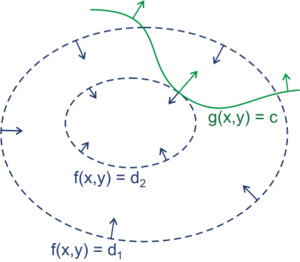
\includegraphics[scale=0.6]{1.png}
\caption{Contours of $\mathbf{g}$ and $\mathbf{f}$ }
\end{figure} 
Denote the function we wish to minimize as $f(\mathbf{w}) = -\mathbf{w}^\mathrm{T} \mathbf{S}_b\mathbf{w}$, and the constraint function as  $g(\mathbf{w}) =  \mathbf{w}^\mathrm{T} \mathbf{S}_w\mathbf{w} - 1 $. 
Then, we should find a stationary point where $f(\mathbf{w}) $ doesn't change along the contours\footnotemark  of $g(\mathbf{w}) = 0$ (Otherwise, then we can follow the direction where $\nabla_{\mathbf{w}}f < 0 $ and get a smaller value ).   In this case, the contour lines of $\mathbf{g}$ and $\mathbf{f}$ must be parallel, which indicates that the derivatives of $\mathbf{g}$ and $\mathbf{f}$ are also parallel \footnotemark.  Therefore: 
\begin{equation}
\nabla_{\mathbf{w}} f + \lambda \nabla_{ \mathbf{w}} g = 0
\end{equation}
Since 
\begin{equation}
 \nabla_{\mathbf{w}} f = - \frac{ \partial}{\partial\mathbf{w} }\mathbf{w}^\mathrm{T} \mathbf{S}_b\mathbf{w}  = - (\mathbf{S}_b + \mathbf{S}_b^T) \mathbf{w} = -2 \mathbf{S}_b \mathbf{w} 
 \end{equation}
 
 \begin{equation}
 \lambda \nabla_{ \mathbf{w}} g = \lambda \frac{ \partial}{\partial\mathbf{w} }  (  \mathbf{w}^\mathrm{T} \mathbf{S}_w\mathbf{w} - 1) =\lambda (\mathbf{S}_w+ \mathbf{S}_w^T) \mathbf{w} = 2  \lambda\mathbf{S}_w \mathbf{w}
 \end{equation}
Combine them together, we have 
  \begin{equation}
  \mathbf{S}_b\mathbf{w} = \lambda \mathbf{S}_w\mathbf{w}
   \end{equation}
To prove that  the solution to equation \eqref{dual} is equivalent to that in equation \eqref{primal},  we  introduce the auxiliary $\mathcal{L}(x,y,\lambda)$: 
 \begin{equation} 
\mathcal{L}(\mathbf{w},\lambda) = f(\mathbf{w}) - \lambda \cdot g(\mathbf{w})
 \end{equation}
Therefore
  \begin{equation} 
 \nabla_{\mathbf{w}, \lambda} \mathcal{L}(\mathbf{w}, \lambda)=0.\iff
 \begin{cases}
\nabla_{\mathbf{w}} f(\mathbf{w}) = \lambda \nabla_{\mathbf{w}} g(\mathbf{w})\\
 g(\mathbf{w}) = 0
\end{cases}
 \end{equation}
 If  $g(\mathbf{w}) = 0$, then the min value of $ \mathcal{L}(\mathbf{w})$ indicates the min value of $f(\mathbf{w})$. 
Since we already have $\nabla_{\mathbf{w}} f(\mathbf{w}) = \lambda \nabla_{\mathbf{w}} g(\mathbf{w})$, whenever $g(\mathbf{w}) = 0$, we result value $\mathbf{w}$ in $\min_{\mathbf{w}}\mathcal{L}(\mathbf{w}) $ is equivalent to that in \eqref{primal}.
 
\footnotetext[1]{Image Reference: https://cuhkmath.wordpress.com/2010/10/12/understanding-lagrange-multipliers/ }
\footnotetext[2]{ \href{https://www.wikiwand.com/en/Lagrange_multiplier}{Wikipedia - Lagrange multiplier}}


~\\
~\\
~\\
~\\
~\\
\qed
\end{prove}

\section{[20pts] Multi-Class Logistic Regression}
教材的章节3.3介绍了对数几率回归解决二分类问题的具体做法。假定现在的任务不再是二分类问题,而是多分类问题,其中$y\in\{1,2\dots,K\}$。请将对数几率回归算法拓展到该多分类问题。

(1) \textbf{[10pts]} 给出该对率回归模型的“对数似然”(log-likelihood);

(2) \textbf{[10pts]} 计算出该“对数似然”的梯度。

提示1:假设该多分类问题满足如下$K-1$个对数几率,
\begin{eqnarray*}
\ln\frac{p(y=1|\mathbf{x})}{p(y=K|\mathbf{x})}&=&\mathbf{w}_1^\mathrm{T}\mathbf{x}+b_1\\
\ln\frac{p(y=2|\mathbf{x})}{p(y=K|\mathbf{x})}&=&\mathbf{w}_2^\mathrm{T}\mathbf{x}+b_2\\
&\dots&\\
\ln\frac{p(y={K-1}|\mathbf{x})}{p(y=K|\mathbf{x})}&=&\mathbf{w}_{K-1}^\mathrm{T}\mathbf{x}+b_{K-1}
\end{eqnarray*}

提示2:定义指示函数$\mathbb{I}(\cdot)$,
$$\mathbb{I}(y=j)=
\begin{cases}
1& \text{若$y$等于$j$}\\
0& \text{若$y$不等于$j$}
\end{cases}$$

\begin{solution} $\,$ \newline
(1) We can run $K-1$ binary logistic regression model, where the $K$th outcome is chosen as the Pivot (Just as the Hint suggests). Therefore:
 \begin{equation}
\begin{split}
\Pr(y=1| \mathbf{x}) &= {\Pr(y=K|\mathbf{x})}e^{ \mathbf{w}_1^\mathrm{T}\mathbf{x}+b_1} \\
\Pr(y=2| \mathbf{x}) &= {\Pr(y=K|\mathbf{x})}e^{ \mathbf{w}_2^\mathrm{T}\mathbf{x}+b_2} \\
\cdots & \cdots \\
\Pr(y=K-1| \mathbf{x}) &= {\Pr(y=K|\mathbf{x})}e^{\mathbf{w}_{K-1}^\mathrm{T}\mathbf{x}+b_{K-1}} \\
\end{split}
\end{equation}

Since the sum of all above possibilities equals to 1, we get:
 \begin{equation}
\begin{split}
\Pr(y=1 | \mathbf{x}) &= \frac{e^{ \mathbf{w}_1^\mathrm{T}\mathbf{x}+b_1}}{1 + \sum_{k=1}^{K-1} e^{\mathbf{w}_k^\mathrm{T}\mathbf{x}+b_k }} \\
\Pr(y=2 | \mathbf{x}) &= \frac{e^{\mathbf{w}_2^\mathrm{T}\mathbf{x}+b_2}}{1 + \sum_{k=1}^{K-1} e^{\mathbf{w}_k^\mathrm{T}\mathbf{x}+b_k }} \\
\cdots & \cdots \\
\Pr(y=K-1|\mathbf{x}) &= \frac{e^{\mathbf{w}_{K-1}^\mathrm{T}\mathbf{x}+b_{K-1}}}{1 + \sum_{k=1}^{K-1} e^{\mathbf{w}_k^\mathrm{T}\mathbf{x}+b_k }} \\
\Pr(y=K|\mathbf{x}) &= \frac{1}{1 + \sum_{k=1}^{K-1} e^{\mathbf{w}_k^\mathrm{T}\mathbf{x}+b_k }} 
\end{split}
\end{equation}
Therefore, let $\mathbf{\boldsymbol\beta_i} = (\mathbf{w_i};b_i)$ and $\mathbf{\hat{x}_i} = (\mathbf{x_i}; 1)$, given dataset $D  = \{(\mathbf{x}_i, y_i) \}_{i=1}^{m}$ the log-likelihood should be:
 \begin{equation}
 \ell(\mathbf{\boldsymbol\beta}) = \sum_{t=1}^{m} \big( \sum_{k=1}^{K-1} \mathbb{I}(y_t = k) \mathbf{\boldsymbol\beta_k}^T\mathbf{\hat{x}_t} - \ln(1 + \sum_{k=1}^{K-1} e^{\mathbf{\boldsymbol\beta_k}^T\mathbf{\hat{x}_t }}) 		\big)
 \end{equation}

(2) The derivative is 
\begin{equation}
\frac{\partial \ell(\boldsymbol\beta)} {\partial \boldsymbol\beta_i }  = \sum_{t=1}^{m} \big(  \mathbb{I}(y_t = i)\mathbf{\hat{x}_t} 
- \mathbb{I}(y_t \neq K)  \frac 
{\mathbf{\hat{x}_t } \cdot e^{\mathbf{\boldsymbol\beta_i}^T\mathbf{\hat{x}_t }} 	}
{1 + \sum_{k=1}^{K-1} e^{\mathbf{\boldsymbol\beta_k}^T\mathbf{\hat{x_t} }}}
\big)
\end{equation}
~\\
~\\
~\\
~\\
~\\
\end{solution}

\section{[35pts] Logistic Regression in Practice} 
对数几率回归(Logistic Regression, 简称LR)是实际应用中非常常用的分类学习算法。

(1) \textbf{[30pts]} 请编程实现二分类的LR, 要求采用牛顿法进行优化求解, 其更新公式可参考《机器学习》教材公式(3.29)。详细编程题指南请参见链接:\url{http://lamda.nju.edu.cn/ml2017/PS2/ML2_programming.html}

(2) \textbf{[5pts]} 请简要谈谈你对本次编程实践的感想(如过程中遇到哪些障碍以及如何解决, 对编程实践作业的建议与意见等)。
\begin{solution}
(2) The problem of Overflow and Underflow happens a lot. Take the sigmoid function as an example, when -x is sufficiently large, \texttt{np.exp(-x)} would raise \texttt{Overflow Exception}. To avoid this, I re-write the function in Python as follows:
\begin{verbatim}
def sigmoid(x):
    max_elem = max(-x) 
    try: 
        	ans = np.exp(-(np.log(np.exp(0 - max_elem) + np.exp(- x - max_elem)) + max_elem ) )
    except Exception as e:
        ans = 0
    return res
\end{verbatim}
The principle behind is:
\begin{equation}
\log{(e^a + e^b)} = \log{(e^{a-m} + e^{b-m})} + m
\end{equation}
Then only underflow would happen. In this case, since the value is sufficiently low, we dismiss the exception and set \texttt{ans} to 0.

\end{solution}
Another problem evolves the \texttt{SingularMatrix Exception}  when running  \texttt{np.linalg.inv(hess)}. Therefore, we could catch the exception and try to determine whether Hessian matrix is too small, if it does not(which means result has't converged), we alternate to gradient descent.
\begin{verbatim}
        try:
            inv = np.linalg.inv(hess)
            beta -= np.matmul(inv, grad(X, beta, y))
        except Exception as e:
            if(np.max(hess) < np.exp(-100)):
                break
            else:
                beta = beta_save - grad(X, beta, y)
\end{verbatim}
The third problem is about the initial value of $w$. When set to all ones, the training algorithm would never converge. This problem was finally found and fixed by setting $w$ to all zeros, after debugging in the dormitory for a whole spring morning ;\_;.
\section{[35pts] Linear Regression with Regularization Term}

给定数据集$D = \{(\mathbf{x}_1,y_1),(\mathbf{x}_2,y_2),\cdots,(\mathbf{x}_m,y_m)\}$, 其中$\mathbf{x}_i = (x_{i1};x_{i2};\cdots;x_{id}) \in \mathbb{R}^d$, $y_i \in \mathbb{R}$, 当我们采用线性回归模型求解时, 实际上是在求解下述优化问题:
\begin{equation}
\label{eq:ls}
\hat{\mathbf{w}}_{\textbf{LS}}^* = \mathop{\arg\min}_{\mathbf{w}} \frac{1}{2}\lVert \mathbf{y} - \mathbf {X}\mathbf{w} \rVert_2^2,
\end{equation}
其中, $\mathbf{y} = [y_1,\cdots,y_m]^\mathrm{T} \in \mathbb{R}^m, \mathbf{X} = [\mathbf{x}_1^\mathrm{T};\mathbf{x}_2^\mathrm{T};\cdots;\mathbf{x}_m^\mathrm{T}]\in \mathbb{R}^{m\times d}$, 下面的问题中, 为简化求解过程, 我们暂不考虑线性回归中的截距(intercept)。

在实际问题中, 我们常常不会直接利用线性回归对数据进行拟合, 这是因为当样本特征很多, 而样本数相对较少时, 直接线性回归很容易陷入过拟合。为缓解过拟合问题, 常对公式\eqref{eq:ls}引入正则化项, 通常形式如下:

\begin{equation}
\label{eq:ls-regular}
\hat{\mathbf{w}}_{\textbf{reg}}^* = \mathop{\arg\min}_{\mathbf{w}} \frac{1}{2}\lVert \mathbf{y} - \mathbf X \mathbf{w} \rVert_2^2 +\lambda \Omega(\mathbf{w}),
\end{equation}
其中, $\lambda> 0$为正则化参数, $\Omega(\mathbf{w})$是正则化项, 根据模型偏好选择不同的$\Omega$。

下面, 假设样本特征矩阵$\mathbf{X}$满足列正交性质, 即$\mathbf{X}^\mathrm{T}\mathbf{X} = \mathbf{I}$, 其中$\mathbf{I}\in \mathbb{R}^{d\times d}$是单位矩阵, 请回答下面的问题(需要给出详细的求解过程):

(1) \textbf{[5pts]} 考虑线性回归问题, 即对应于公式\eqref{eq:ls}, 请给出最优解$\hat{\mathbf{w}}_{\textbf{LS}}^*$的闭式解表达式;

(2) \textbf{[10pts]} 考虑\href{https://en.wikipedia.org/wiki/Tikhonov_regularization}{岭回归(ridge regression)}问题, 即对应于公式\eqref{eq:ls-regular}中$\Omega(\mathbf{w}) = \lVert \mathbf{w}\rVert_2^2=\sum_{i=1}^d w_i^2$时, 请给出最优解$\hat{\mathbf{w}}_{\textbf{Ridge}}^*$的闭式解表达式;

(3) \textbf{[10pts]} 考虑\href{https://en.wikipedia.org/wiki/LASSO}{LASSO}问题, 即对应于公式\eqref{eq:ls-regular}中$\Omega(\mathbf{w}) = \lVert \mathbf{w}\rVert_1=\sum_{i=1}^d \vert w_i\vert$时, 请给出最优解$\hat{\mathbf{w}}_{\textbf{LASSO}}^*$的闭式解表达式;

(4) \textbf{[10pts]} 考虑$\ell_0$-范数正则化问题, 
\begin{equation}
\label{eq:ls-l0}
\hat{\mathbf{w}}_{\mathbf{\ell_0}}^* = \mathop{\arg\min}_{\mathbf{w}} \frac{1}{2}\lVert \mathbf{y} - \mathbf X \mathbf{w} \rVert_2^2 +\lambda \lVert \mathbf{w}\rVert_0,
\end{equation}
其中, $\lVert \mathbf{w}\rVert_0=\sum_{i=1}^d \mathbb{I}[w_i \neq 0]$,即$\lVert \mathbf{w}\rVert_0$表示$\mathbf{w}$中非零项的个数。通常来说, 上述问题是NP-Hard问题, 且是非凸问题, 很难进行有效地优化得到最优解。实际上, 问题(3)中的LASSO可以视为是近些年研究者求解$\ell_0$-范数正则化的凸松弛问题。

但当假设样本特征矩阵$\mathbf{X}$满足列正交性质, 即$\mathbf{X}^\mathrm{T}\mathbf{X} = \mathbf{I}$时, $\ell_0$-范数正则化问题存在闭式解。请给出最优解$\hat{\mathbf{w}}_{\mathbf{\ell_0}}^*$的闭式解表达式, 并简要说明若去除列正交性质假设后, 为什么问题会变得非常困难?

\begin{solution} $\,$ \newline
(1)  Let 
\begin{equation}
\begin{split}
J(\mathbf{w}) &= \frac{1}{2} \lVert \mathbf{y} - \mathbf {X}\mathbf{w} \rVert_2^2 = \frac{1}{2} (\mathbf{Xw-y})^T(\mathbf{Xw-y}) \\
&= \frac{1}{2}  (\mathbf{	(Xw)^TXw-(Xw)^Ty-y^T(Xw)+y^Ty	})
\end{split}
\end{equation}
Since
\begin{equation}
\label{J:s}
\frac{\partial J}{\partial\mathbf{w}}=\mathbf{X^TXw-X^{T}y}
\end{equation}
Let  \eqref{J:s} = 0, since $\mathbf{X}^\mathrm{T}\mathbf{X} = \mathbf{I}$, we have
\begin{equation}
\mathbf{w}=\mathbf{(X^T X)^{-1}X^T y} = \mathbf{X^T y}
\end{equation}
~\\
(2)	Let 
\begin{equation}
\begin{split}
J(\mathbf{w}) &= \frac{1}{2}\lVert \mathbf{y} - \mathbf X \mathbf{w} \lambda \rVert_2^2 + \lVert \mathbf{w}\rVert_2^2 \\
&= \frac{1}{2} (\mathbf{(Xw)^TXw-2(Xw)^Ty+y^Ty)	 + \lambda w^Tw}
\end{split}
\end{equation}
Since
\begin{equation}
\label{J:s-norm}
\frac{\partial J}{\partial\mathbf{w}}=\mathbf{X^TXw-X^{T}y + 2 \lambda w}
\end{equation}
Let  \eqref{J:s-norm} = 0, we have
\begin{equation}
\mathbf{w}=\mathbf{(X^T X + 2\lambda I_d)^{-1}X^T y}  = \mathbf{\frac{1}{1 +2 \lambda}X^T y} 
\end{equation}
~\\
\newcommand{\wls}{\hat{\mathbf{w}}^{{\small \text{LS}}}}
\newcommand{\boldw}{\mathbf{w}}
\newcommand{\wlasso}{\hat{\mathbf{w}}^{{\text{lasso}}}} 
(3) Let $\wls$ denote the solution to \eqref{eq:ls}($\textit{i.e.}$ $\wls = \mathbf{X^T y}$), we have:
\begin{equation}
\begin{split}
J(\mathbf{w})  &=  \frac{1}{2} \| \mathbf{y - X w} \|_2^2 + \lambda \| \mathbf{w}\|_1   \\
&=  \frac{1}{2} (\mathbf{w^TX^TXw-2(Xw)^Ty+y^Ty)	 + \lambda  \| \mathbf{w}\|_1  }  \\
&=  \frac{1}{2} (\mathbf{\sum_{i=1}^{d} w_i^2 - 2wX^Ty+y^Ty)	 + \lambda  \| \mathbf{w}\|_1  } \\
&=  \frac{1}{2} (\mathbf{\sum_{i=1}^{d} (w_i^2 - 2w_i \wls_i) + y^Ty)	 + \lambda  \| \mathbf{w}\|_1  } 
\end{split}
\end{equation}
Since $\mathbf{y^Ty}$ is irrelevant to $\mathbf{w}$ we have it discarded. Therefore:
\begin{equation}
\min_{\boldw}J(\mathbf{w})  =\min_{\boldw} \sum_{i=1}^{d}(\frac{1}{2} \boldw_i^2 - \boldw_i \wls_i +  \lambda |\mathbf{\boldw_i}|) 
\end{equation}
Where $\boldw_i$ is independent to $\boldw_j (i \neq j)$, and we can minimize the whole $J(\mathbf{w})$ by finding $\boldw_k (k = 1, 2, 3 ..., d)$ one by one, $\textit{i.e}$. for every $k \in [1, d]$, we need to find
\begin{equation} 
\min_{\boldw_k}J(\boldw_k) = \min_{\boldw_k} (\frac{1}{2} \boldw_k^2 - \boldw_k \wls_k +  \lambda |\mathbf{\boldw_k}|)
\end{equation}
Since the value of $\frac{1}{2} \boldw_k^2$ and $\lambda |\mathbf{\boldw_k}|$ is independent to the sign, if  $\wls_k > 0$ then $\boldw_k$ must be $\geq 0$.  If $\wls_k \leq 0$ then $\boldw_k \leq 0$. 
Then:
\begin{equation} 
\label{J:w_k}
J(\boldw_k) = \left\{ \begin{array}{ll}
 \frac{1}{2} \boldw_k^2 - \boldw_k \wls_k +  \lambda \boldw_k & ,\wls_k > 0 \\
\frac{1}{2}  \boldw_k^2 - \boldw_k \wls_k -  \lambda  \boldw_k  &,\wls_k \leq 0
  \end{array} \right.
\end{equation}
In either case, we have:
\begin{equation}
\frac{\partial J(\boldw_k)}{\partial\mathbf{w_k}} = \boldw_k -  \wls_k +  \text{sign}(\wls_k) \cdot \lambda
\end{equation}
Therefore, the closed-form solution is given by:\footnotemark
\begin{equation}
\wlasso_k = \left\{ \begin{array}{ll}
\wls_k - \text{sign}(\wls_k) \cdot \lambda &, \lambda < |\wls_k| \\
0  &, \lambda > |\wls_k|
  \end{array} \right.
\end{equation}
\newcommand{\wlz}{\hat{\mathbf{w}}^{\ell_0}}
(4) Let
\begin{equation}
\begin{split}
J(\mathbf{w})   &=  \frac{1}{2} (\mathbf{(\sum_{i=1}^{d} (w_i^2 - 2w_i \wls_i) + y^Ty)	 + \lambda  \| \mathbf{w}\|_0  } 
\end{split}
\end{equation}
Similar to \eqref{J:w_k}, we have: 
\begin{equation} 
J(\boldw_k) = \left\{ \begin{array}{ll}
0  & ,\boldw_k = 0 \\
\frac{1}{2}  \boldw_k^2 - \boldw_k \wls_k +  \lambda  &,\boldw_k \neq 0
 \end{array} \right.
\end{equation}
Therefore, from basic principles of the quadratic equation, we have
\begin{equation}
\wlz_k = \left\{ \begin{array}{ll}
\wls_k  &,  (\wls_k)^2  - 2\lambda > 0 \\
0  								&,  (\wls_k)^2  - 2\lambda \leq 0
  \end{array} \right.
\end{equation}
The orthonormality of $\mathbf{X}$ generally assumes the independency between columns of $\wlz$ . if $\mathbf{X}$  is non-orthonormal,   the $L0$-penalty makes the solution non-convex,   which is NP-hard in general.
 \footnotemark   
~\\
~\\
\end{solution}

\footnotetext[3]{ C Leng.  A note on the Lasso in Model Selection Statistica Sinica 16(2006), 1273-1284}
\footnotetext[4]{Cedric E. Ginestet,  Regularization: Ridge Regression and Lasso,  Boston University, MA 575 Linear Models, Week 14, Lecture 2}
\end{document}